\documentclass[tikz]{standalone}

\usepackage{pgfplots}
\pgfplotsset{compat=newest}

\tikzset{
    canvas/.style={draw,left color=blue!35!black,right color=white},
    sign/.style={align=center,fill=white,fill opacity=0.2,text opacity=1,text=white},
    axis label/.style={midway,below,sloped}
}

\def\datapoint(#1,#2,#3)(#4) {
    \filldraw (#1,#2,#3) -- (#1,#2,0) circle (0.2ex) (#1,#2,#3) -- (0,#2,#3) circle (0.2ex) (#1,#2,#3) -- (#1,0,#3) circle (0.2ex);
    \shade[ball color=blue!40] (#1,#2,#3) circle (1ex) node[sign,right=1ex] {#4};}

\begin{document}

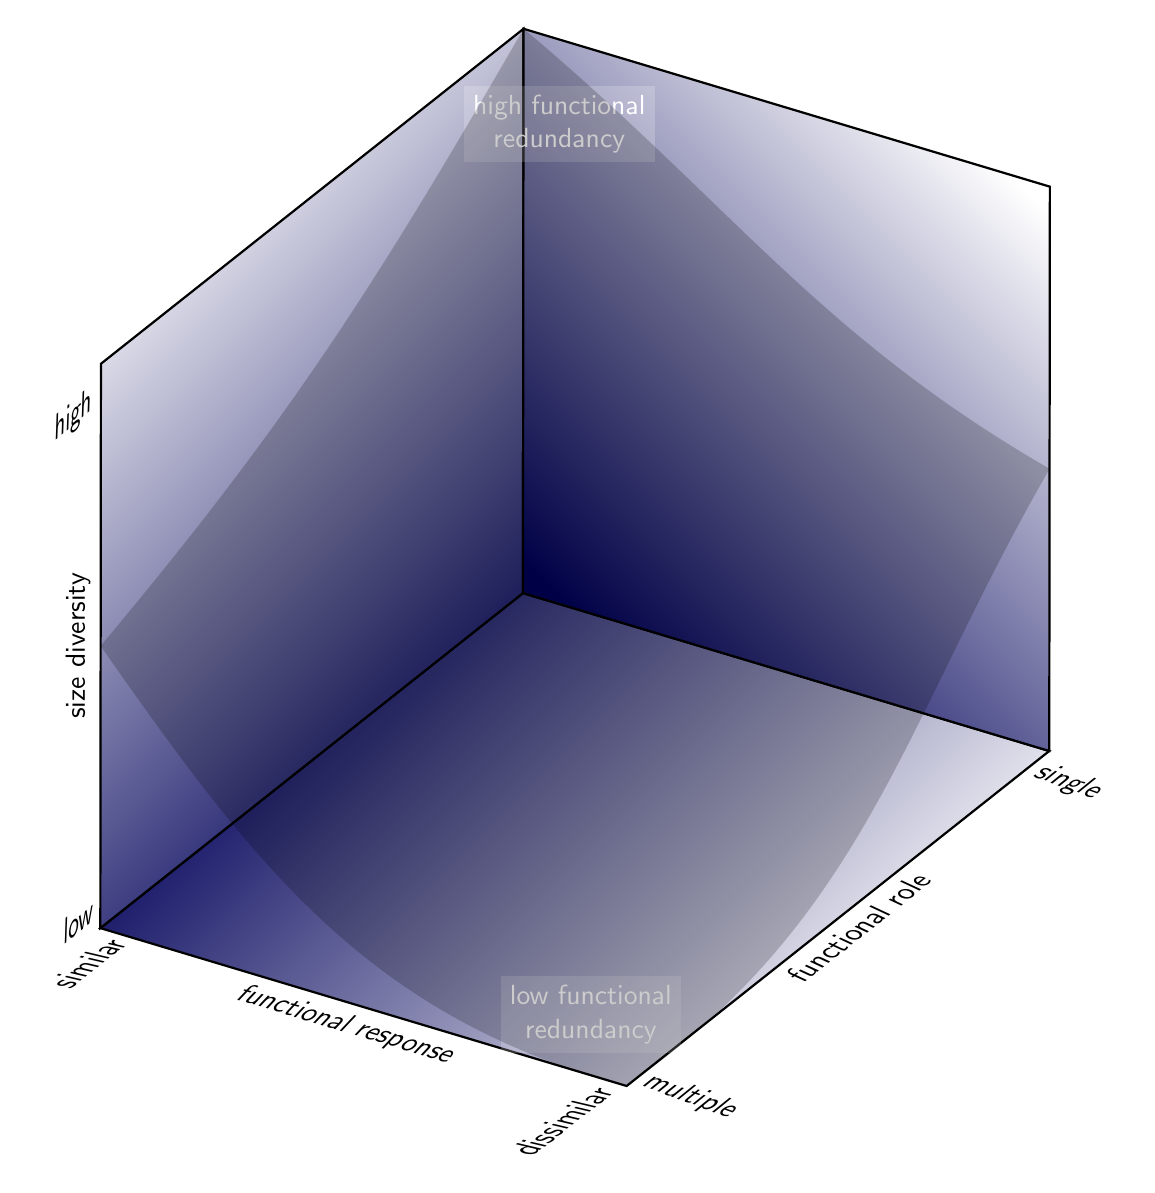
\begin{tikzpicture}[font=\sffamily,thick,rotate around y=-17,rotate around z=-8,rotate around x=10]

  \shade[canvas,shading angle=45]
  (0,0,0) -- (8,0,0)
  node[below right,rotate=-20,xslant=0.6] {single}
  -- (8,0,8)
  node[right,rotate=-20,xslant=0.6,yshift=1ex] {multiple}
  node[left,rotate=38,xslant=-0.8,yshift=1ex] {dissimilar}
  node[sign,shift={(-3ex,6ex)}] {low functional\\redundancy}
  node[axis label,xslant=-0.5] {functional role}
  -- (0,0,8)
  node[axis label,xslant=0.5] {functional response}
  node[below left,rotate=38,xslant=-0.8] {similar}
  -- cycle;

  \shade[canvas,shading angle=225]
  (0,0,0) -- (0,0,8)
  node[above left,rotate=40,xslant=0.9] {low}
  -- (0,8,8)
  node[axis label,above] {size diversity}
  node[below left,rotate=40,xslant=0.9] {high}
  -- (0,8,0)
  -- cycle;

  \shade[canvas,shading angle=135]
  (0,0,0) -- (8,0,0)
  -- (8,8,0)
  -- (0,8,0)
  node[sign,shift={(3ex,-8ex)}] {high functional\\redundancy}
  -- cycle;

  \datapoint(4,0.5,6)(DIATOM)
  \datapoint(5,1,3)(DIAZO)
  \datapoint(3,1.5,2)(PHAEO)
  \datapoint(4.5,4,4.5)(COCCO)
  \datapoint(5.5,7,3.5)(PICO)

  \fill[opacity=0.2] (8,0,8) to[out=35,in=-120] (8,4,0) to[out=150,in=-40] (0,8,0) to[out=-120,in=50] (0,4,8) to[out=-55,in=165] cycle;

\end{tikzpicture}
\end{document}
